%------------------------------------------------------------------------------
% Author(s):
% Varaun Ramgoolie
% Copyright:
%  Copyright (C) 2020 Brad Bachu, Arjun Mohammed, Nicholas Sammy, Kerry Singh
%
%  This file is part of Applied-Mathematics-Unit2 and is distributed under the
%  terms of the MIT License. See the LICENSE file for details.
%
%  Description:
%     Year: 2006 C
%     Module: 1
%     Question: 2
%------------------------------------------------------------------------------
\usetikzlibrary{patterns}

\begin{subquestions}
	
%------------------------------------------------------------------------------
% 2 a -------------------------------------------------------------------------
%------------------------------------------------------------------------------

\subquestion

Let us define $x$ as "the number of large trucks used" and $y$ as "the number of small trucks used". The objective function that we want to minimize is,

\begin{equation}
	C = 240x + 100y \,.
\end{equation}

The constraints in this linear programming model are as follows,

\begin{align}
	12(5x + 2y) & \geq 1200 \,, \nn \\
	x + y & \leq 50 \,, \nn \\
	x & \leq 25 \,, \nn \\
	y & \geq 15 \,. 
\end{align}

%------------------------------------------------------------------------------
% 2 b -------------------------------------------------------------------------
%------------------------------------------------------------------------------

\subquestion

\begin{subsubquestions}

%------------------------------------------------------------------------------
	
\subsubquestion

See the graph below. 

\begin{center}
	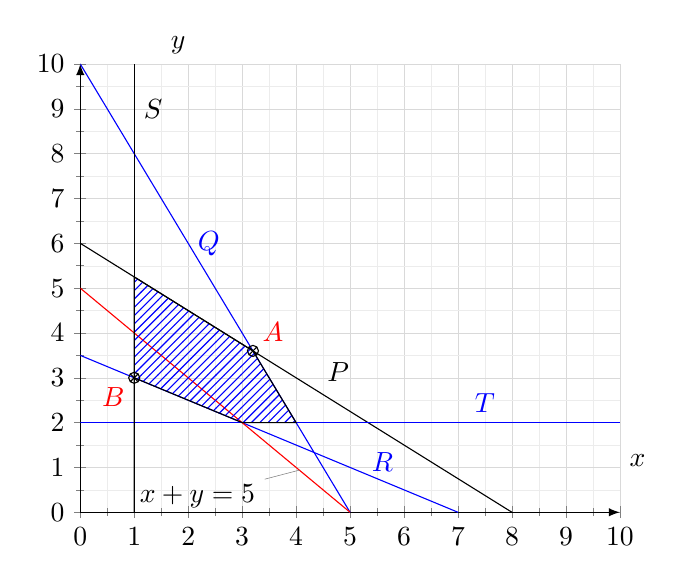
\begin{tikzpicture}
		\begin{axis}
			[
			xmin=-0,xmax=10,
			ymin=0,ymax=10,
			grid=both,
			grid style={line width=.1pt, draw=darkgray!10},
			major grid style={line width=.2pt,draw=darkgray!20},
			axis lines=left,
			minor tick num=1,
			enlargelimits={abs=0},
			axis line style={-latex},
			samples=100,
			domain = -20:20,
			ytick={0,1,...,10},
			xtick={0,1,...,10},
			xlabel={$x$},
			ylabel={$y$},
			x label style={at={(axis description cs:1,0.15)},anchor=north west},
			y label style={at={(axis description cs:0.15,1)},anchor=south west, rotate=-90}
			]
		
			\addplot [mark=dot,blue] coordinates{(5, 0)  (0,10)}	node[pos=0.6,blue, right] {$Q$};
			
			\addplot [mark=dot,blue] coordinates {(7,0) (0, 3.5)} node[pos=0.2,above,blue] {$R$};
		
			\addplot [mark=dot] coordinates {(8,0) (0, 6)} node[pos=0.45, above right] {$P$};
			
			\addplot [mark=dot] coordinates {(1,0) (1, 10)} node[pos=0.90, right] {$S$};
			
			\addplot [mark=dot, blue] coordinates {(0,2) (10, 2)} node[pos=0.75,above, blue] {$T$};
			
			\addplot [mark=dot, red] coordinates {(5,0) (0, 5)};
			
			\node [pin=190:{$x+y=5$}] at (axis cs:(4.25, 1) {};
			
			\addplot [pattern=north east lines,pattern color=blue] coordinates {(1,3) (3, 2) (4, 2) (3.2,3.6) (1, 5.25)} \closedcycle;	
			
			\addplot [mark=otimes] coordinates{(1, 3)} node[below left, red] {$B$};
			
			\addplot [mark=otimes] coordinates{(3.2, 3.6)} node[above right, red] {$A$};
		
		\end{axis}	
	\end{tikzpicture}
\end{center}

%--------------------------------------------------------------------------------

\subsubquestion

The feasible region is shaded in the graph.

%--------------------------------------------------------------------------------

\subsubquestion

The line, $x+y=5$, is the red line in the graph. Both $A$ and $B$ are also labeled on the graph.

\end{subsubquestions}

\end{subquestions}
